\section{问题四的分析与求解}

\instruction{本节占位。问题四：引入失水收缩导致的移动边界（附录 4 变物性 + 尺寸变化，半径 \R 随时间变化）。建议坐标变换到固定计算域（如 $\xi = r/R(t)$），该建模决策需记入 docs/DECISIONS.md。由 @model 提供公式、@impl 求解、@paper 排版。}

\subsection{模型的建立}
\instruction{移动边界控制方程、坐标变换、变物性参数化占位。}

\subsection{模型的求解}
\instruction{固定计算域离散、移动边界处理策略占位。}

\subsection{结果与分析}
\instruction{结果表/图由 scripts 生成。result4.xlsx 仅含水分浓度（工作表名 Sheet1），末列「药材表面」为当时的表面位置（见 AGENTS.md §5）。}

% 表格片段本身已是完整的 table 环境，不再套一层（见 05_q2.tex 的说明）。
% 表 6 的末列是「药材表面」＝当时的表面位置，由 make_tables.py 从 csv 原样带入。
\IfFileExists{tab/q4_moist.tex}{%
  % 本文件由 scripts/make_tables.py 自动生成，请勿手工编辑
\begin{table}[htbp]
  \centering
  \caption{考虑收缩的药材烘干过程的水分浓度（kg/kg；距离单位：cm）}
  \label{tab:q4-moisture}
  \begin{tabular}{cccccc}
    \toprule
    时间/h & 0 & 0.5 & 1 & 1.5 & 药材表面 \\
    \midrule
    6.0000 & 2.4209 & 2.3149 & 1.7826 &  & 0.7059 \\
    12.0000 & 1.2718 & 1.1023 & 0.6297 &  & 0.2357 \\
    18.0000 & 0.5322 & 0.4732 & 0.2908 &  & 0.0798 \\
    24.0000 & 0.3008 & 0.2745 & 0.1856 &  & 0.0266 \\
    30.0000 & 0.2181 & 0.2020 & 0.1447 &  & 0.0119 \\
    36.0000 & 0.1786 & 0.1669 & 0.1237 &  & 0.0067 \\
    42.0000 & 0.1557 & 0.1464 & 0.1111 &  & 0.0043 \\
    44.0360 & 0.1500 & 0.1412 & 0.1078 &  & 0.0037 \\
    \bottomrule
  \end{tabular}
\end{table}
%
}{%
  \instruction{表占位：tab/q4\_moist（scripts/make\_tables.py 生成）尚未生成。}
}

\begin{figure}[htbp]
  \centering
  \IfFileExists{figs/fig4-C-profiles.pdf}{%
    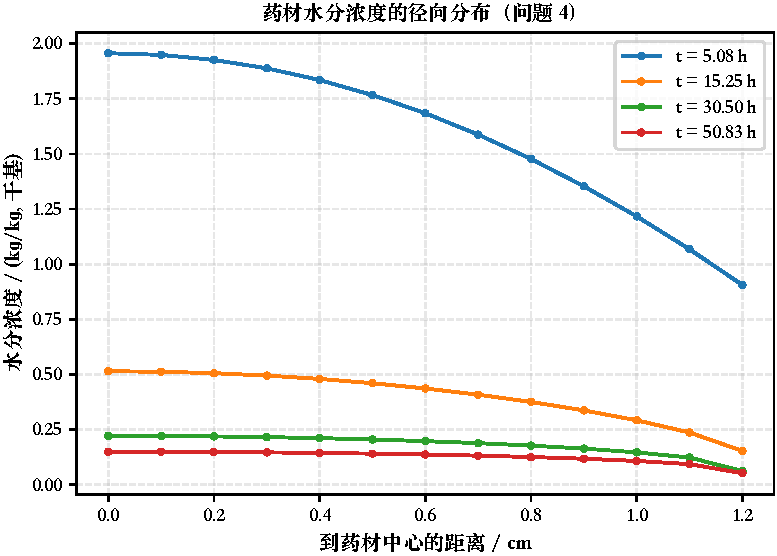
\includegraphics[width=0.75\linewidth]{figs/fig4-C-profiles.pdf}%
  }{%
    \instruction{图占位：figs/fig4-C-profiles.pdf 尚未生成（scripts/make\_figs.py）。}
  }
  \caption{考虑收缩时药材内部水分浓度分布（材料坐标 $\xi=r/R(t)$）}
  \label{fig:q4-concentration}
\end{figure}
